\chapter{Prior Art in Terrain Modeling}
\label{chapter:TerrainRepresentations}



% FOOTNOTE THE ATTRIBUTIONS
\let\thefootnote\relax\footnote{Portions of this chapter previously appeared as: FIX \bibentry{stuetzle-TerrainDistances} }


The variation in GIS applications and the need for faster access and more compressibility 
% for terrain data 
has resulted in the development of a variety of data representations for elevation information. 
% Terrain data can and has been modeled in several ways, depending on the overlying application. 
Some only require that the surface of the terrain be modeled, while others need volumetric data stored as well.

% Real life terrain (deemed, in this thesis, to be the set of \textit{legal terrain}) differs from common data representations in a variety of ways. First, real terrain is not necessarily continuous everywhere. In fact, discontinuities litter the surface of the earth, from cliff faces and waterfalls to caves and tunnels. These discontinuities are difficult to represent with any spatial data structure. Second, because most terrain does not contain local minima, small pits that can collect water and prevent easy travel, legal terrain also lacks local minima. Error is inevitable during the surface data collection phase, and so oftentimes local minima are introduced where there should be none. Spatial datasets allow for this inaccuracy, with no mechanism for minimization or prevention. Thirdly, ideal terrain representations should contain formation information beyond that of strictly the spatiality of the data, closely tying the representation to the physics responsible for generating the terrain. When determining the accuracy and viability of common terrain representations, the ability to model legal terrains should be taken into account. Finally, an ideal terrain representation will allow for local data manipulation without effect on the global shape.

\section{Surface Representations of Terrain}
\label{section:SurfaceRepresentations}

For many applications, knowledge of only the surface of the terrain is sufficient. In computer graphics, surface data is used for many terrain generation techniques, including fractal generation and shallow water erosion simulations.
In each case, individual grid values are manipulated, requiring knowledge of only elevations along the surface. 
Like all models, rendering a terrain requires only the surface data, as well.

The method of terrain representation chosen can have a profound effect on the application it is used for. Walker et al. \cite{elevationDataEffects} demonstrate the way in which inaccurate terrain data may effect a seemingly unrelated application, atmospheric modeling. Small changes (i.e. errors) introduced into the data have a substantial effect on the results of atmospheric models.

% Most applications in computer graphics (terrain generation, rendering, simulation) and GIS (hydrography, dam siting, path planning) require knowledge of only the surface of the terrain. There are many representations that encode only the surface, including height fields, triangulated irregular networks (TINs), and Fourier functions.

\subsection{Height Fields}

\begin{figure}
  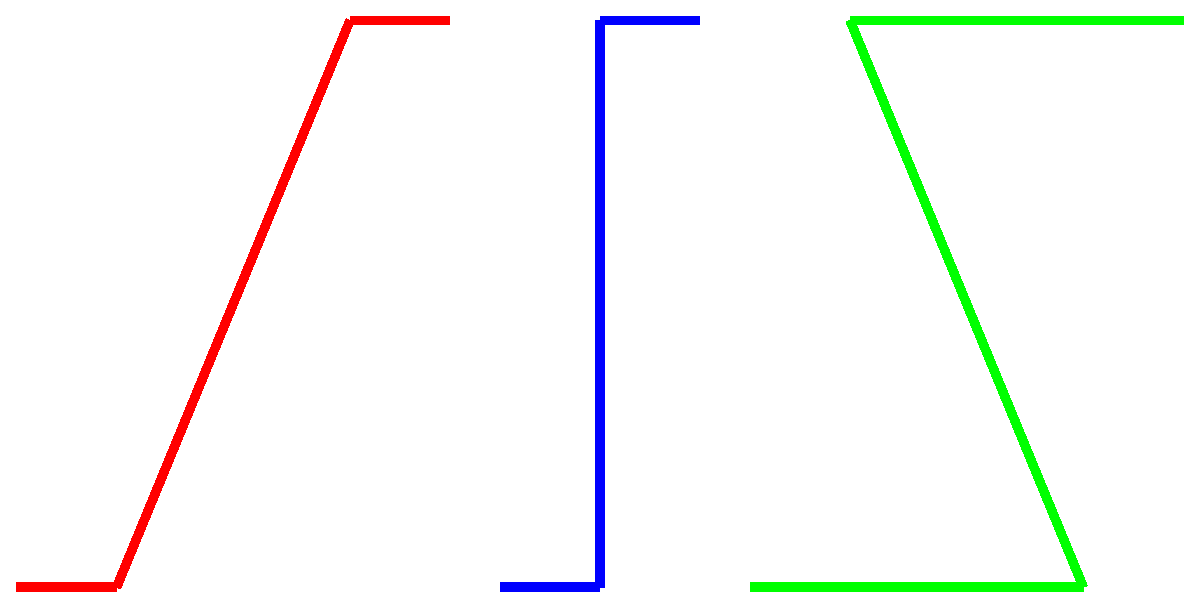
\includegraphics[width=0.99\textwidth]{images/TerrainShapes.eps}
  \caption[Various terrain formations too complex for surface representations]{\label{figure:TerrainShapes}Three possible terrain formations that are indistinguishable given spatial height field data: a positive slope (red), a vertical cliff face (blue), and an overhang (green). These formations are too complex for any surface representation to correctly model.}
\end{figure}

%Figure of each datasets
\begin{figure*}[t]
\centering
\begin{minipage}[b]{0.3\linewidth}
\begin{center}
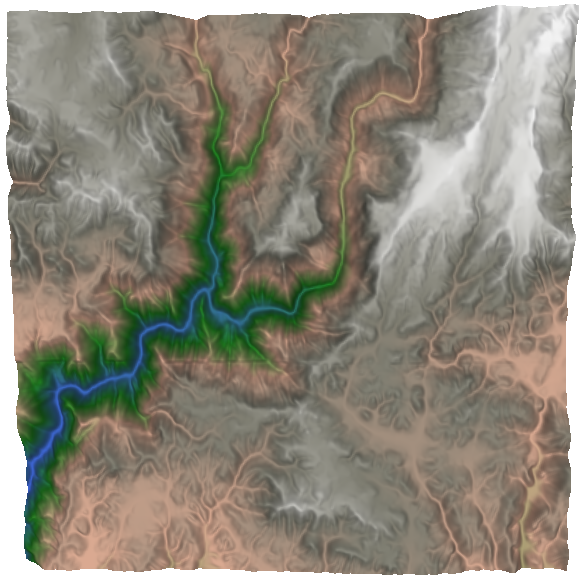
\includegraphics[width=\linewidth]{images/mtn1_normalized.png} \\
MTN1
\end{center}
\end{minipage}
%
\begin{minipage}[b]{0.3\linewidth}
\begin{center}
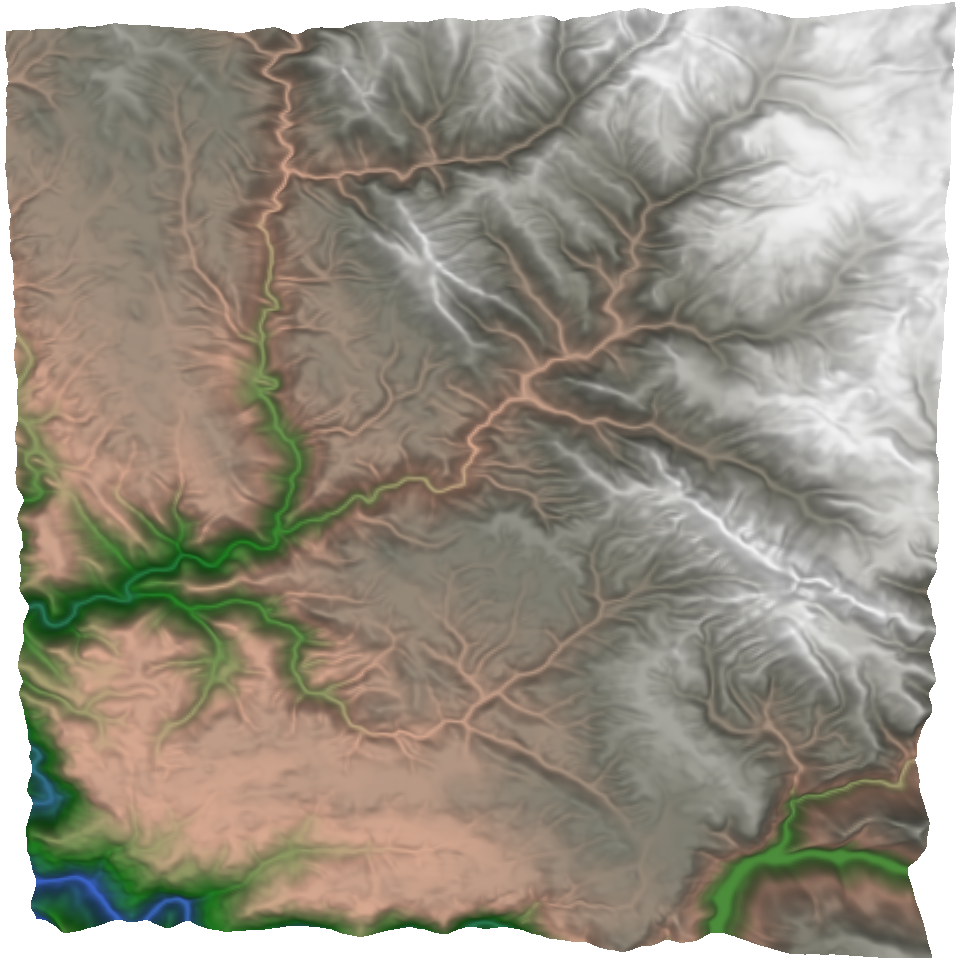
\includegraphics[width=\linewidth]{images/mtn2_normalized.png} \\
MTN2
\end{center}
\end{minipage}
%
\begin{minipage}[b]{0.3\linewidth}
\begin{center}
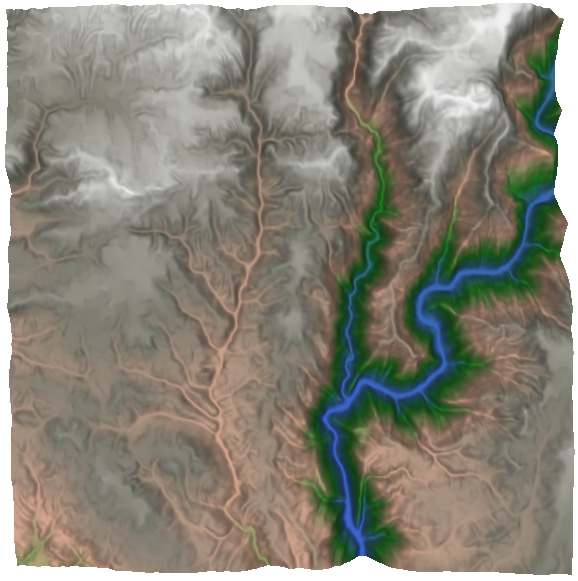
\includegraphics[width=\linewidth]{images/mtn3_normalized.png} \\
MTN3
\end{center}
\end{minipage} \\
%
\begin{minipage}[b]{0.3\linewidth}
\begin{center}
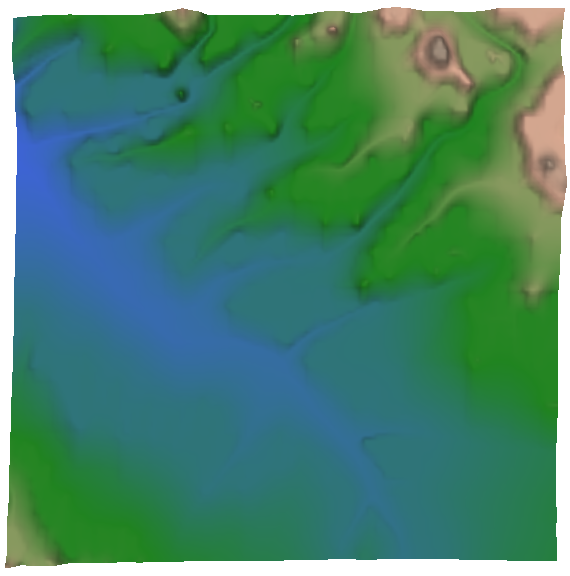
\includegraphics[width=\linewidth]{images/hill1_normalized.png} \\
HILL1
\end{center}
\end{minipage}
%
\begin{minipage}[b]{0.3\linewidth}
\begin{center}
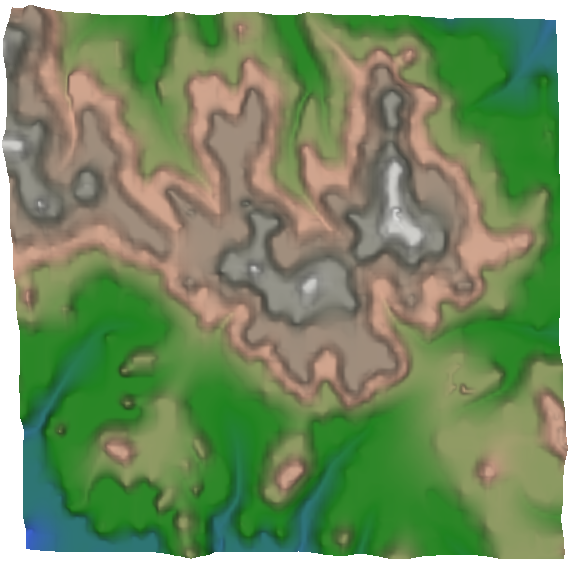
\includegraphics[width=\linewidth]{images/hill2_normalized.png} \\
HILL2
\end{center}
\end{minipage}
%
\begin{minipage}[b]{0.3\linewidth}
\begin{center}
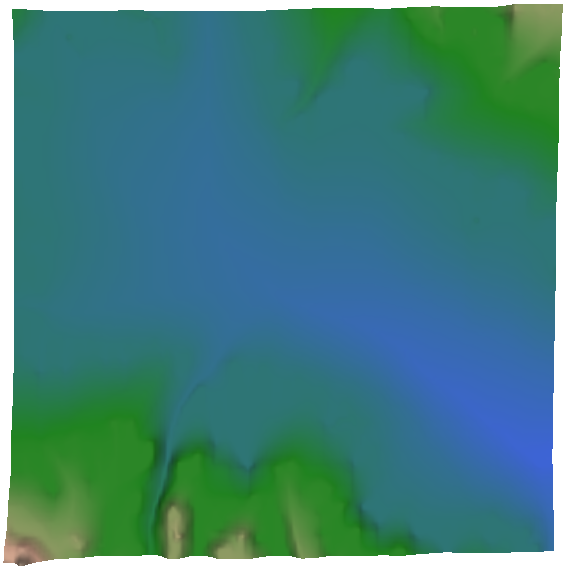
\includegraphics[width=\linewidth]{images/hill3_normalized.png} \\
HILL3
\end{center}
\end{minipage}
%
\caption[Six height field datasets used for analysis]{\label{figure:SixDatasets} Six $400 \times 400$ height fields used in this thesis for analysis, three mountainous datasets (top row) and three hilly datasets (bottom row). These are top-down views of each set, and color indicates elevation (normalized to the maximum elevation range of the set) measured in meters, transitioning from white at the highest elevations, to brown, then green, and then to blue at the lowest elevations. These datasets were first used by Inanc \cite{inanc-phd}.}
\end{figure*}

\begin{table}
\centering
\caption[Geological information regarding six datasets.]{\label{table:SixDatasetsInformation}Geological information regarding the six datasets used in this thesis, presented graphically in Figure \ref{figure:SixDatasets}. This table was first used by Lau and Franklin \cite{Lau-CAGIS}. }
\small{
\begin{tabular}{|c|c c|c c c|}
\hline
               &                  &                     & \multicolumn{3}{c}{Elevation in meters}      \\
DEM 		   & Cell name        & Cell Range          & Mean            & Standard Deviation & Range \\ \hline
\textit{HILL1} & \texttt{W111N31} & 401:800,1:400       & 1251            & 79                 & 1105:1610 \\
\textit{HILL2} & \texttt{W111N31} & 401:800,401:800     & 1548            & 134                & 1198:1943 \\
\textit{HILL3} & \texttt{W111N31} & 401:800,801:1200    & 1309            & 59                 & 1199:1699 \\
\textit{MTN1}  & \texttt{W121N38} & 1201:1600,1201:1600 & 712             & 146                & 219:1040 \\
\textit{MTN2}  & \texttt{W121N38} & 2801:3200,801:1200  & 847             & 152                & 330:1283 \\
\textit{MTN3}  & \texttt{W121N38} & 3201:3600,401:800   & 723             & 161                & 233:1021 \\
\hline
\end{tabular}
}
\end{table}


Height fields are matrices of evenly-spaced elevation values (each x,y coordinate has exactly one corresponding elevation). Each grid space is referred to from this point forward as a pixel. 
% Throughout this work, these elevations will be assumed to be whole integer values.
%  (which is not always the case, but has no 
In most applications in GIS, terrain is stored as a Digital Elevation Model (DEM), whose underlying representation is a height field. Due to their simplicity, height fields are often the least complex representation to work with. Many GIS algorithms have been optimized for elevation grids. The regularity of their grid structure and the simplicity of the representation itself make height fields ideal candidates for most applications, but they have shortcomings as well.

The accuracy of height fields is limited by the assumption that terrain is $C^{0}$ continuous everywhere,
%  and differentiable, 
which is rarely true.
Discontinuities are apparent in real terrain (e.g. the Grand Canyon), but the information necessary to represent them is lost when storing a matrix of elevation values. For instance, given the following matrix of elevations:

\begin{center}
  \begin{tabular}{c|c|c}
    24 & 23 & 12 \\
    \hline
    23 & 21 & 12 \\
    \hline
    24 & 21 & 11 
  \end{tabular} 
\end{center}

\noindent it is impossible to determine whether the slope between columns 2 and 3 is positive, undefined (vertical), or negative (an overhang), and so it is assumed to be positive in most applications. 
Examples of these three possibilities with regard to their surface shape is shown in Figure \ref{figure:TerrainShapes}.
% At coarse grid resolutions, this may force 
For many terrain formations, this is 
% correct, or at least 
sufficient.
% , but not always.

Height field data collection requires acquiring samplings of elevation values. Modern collection processes suffer from failure to adhere to the Nyquist Sampling Theorem \cite{nyquist}, which states that the sampling frequency of a set of data should be at least twice that of the data itself. Due to this and the lack of a representation of terrain that facilitates more accurate data collection, there is a great deal of terrain data that contains inaccuracies.

Figure \ref{figure:SixDatasets} shows a graphical representation of the six height field datasets that are used throughout this thesis. Three mountainous datasets and three hilly datasets are used, each a $400 \times 400$ grid of pixels with elevation values measured in meters. Notice that the mountainous datasets have very clearly defined channels (rivers) running through them, like veins. The hilly datasets, however, are low-frequency data with very few features and large, flat areas. 

\subsection{Triangulated Irregular Networks}

% \fbox{WILL ADD A FIGURE OF A TIN FROM ARCGIS}
 
TINs are triangulated terrain surfaces built of piecewise linear splines, and can be thought of as triangulated 
% grid-less 
three-dimensional points (or nodes) with stored or known connectivity.
TINs are often formed by triangulating a sampled set of points from a height field, thus allowing for a more compact representation.
TINs suffer from the same limitation as height fields because triangulated representations require that each node's (x,y) coordinate be unique and single-valued to generate a continuous surface (i.e., with $C^{0}$ continuity).

In addition, the accuracy of 
both height fields and TINs are dependent almost entirely on the resolution of the data points. Coarser resolutions have a profound and negative effect on the accuracy bound of the data (Gao \cite{gao:resolution}). This limitation can be somewhat mitigated by developing variable resolution, possible for both representations (such as in Abdelguerfi, et al. \cite{Abdelguerfi-HierTINs}, De Floriania, et al. \cite{DeFloriani-HTINs}, Bartholdi and Goldsman \cite{BartholdiAndGoldsman-HierTINs}, and Velho, et al. \cite{Velho-HierTINs}), but even this solution is limited. More data points requires more storage and introduces more sources of possible error. The trade-off of more data points means that finding a TIN-approximation of a given surface is complex. 
In fact, Agarwal and Suri \cite{Agarwal:1994:SAG:314464.314475} show that computing a piecewise linear $\epsilon$-approximation of a bivariate function (terrain surface) is NP-Hard. 

Additional information layers are often stored on top of height fields and TINs. Scalatos and Pavlidis \cite{Scarlatos:1990:HTU:949531.949559} represent hierarchical connectivity information for the TIN, because organizational scheme is important for algorithmic efficiency when using TINs. Similarly, Cignoni et al. \cite{Cignoni97representationand} present a hierarchical method for approximating a TIN with fewer triangles by greedily adding elements to the approximating set one at a time and recalculating the global error. Triangles in this system remember the overall error before and after their ``birth'' and ``death'' allowing for simple optimization.
Keller and Baru \cite{KellyAndBaru_GPLATES} present GPlates, a system for visualizing and manipulating plate tectonic data. The internal representation of the data is as 3D unit vectors, with the poles given [ 0 0 1 ] and [ 0 0 -1 ], to avoid the problem of having to assign a longitude to them. The actual elevation data is simply a height field, and plate boundaries are stored as polygons, or collections of elevation values. Baumann et al. \cite{Baumann:1999:HHD:792758.793044} present a hierarchical data structure that has been generalized for textured terrains. The data structure is essentially a generalization of k-d trees on a gridded terrain that can be applied to other terrain representations, such as TINs.

\subsection{Fourier Series, Splines, and Other Mathematical Models}

% \fbox{ADD AN IMAGE OF EACH KIND OF FUNCTION}

\begin{figure}
  \begin{center}
%     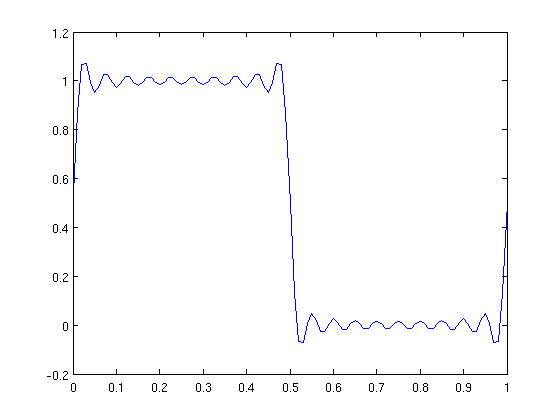
\includegraphics[width=0.5\textwidth]{images/Fourier_N20.png}
    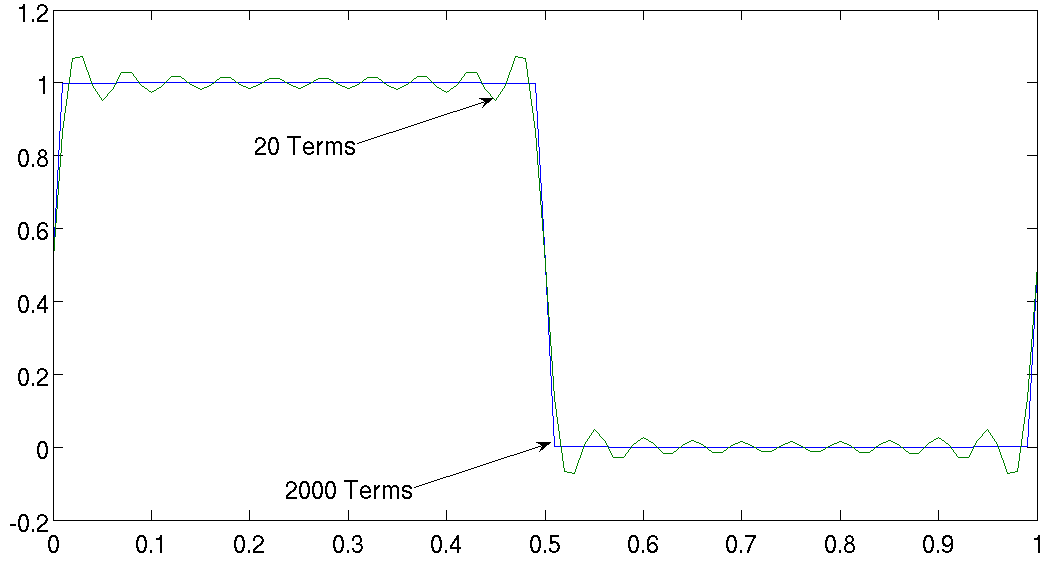
\includegraphics[width=0.75\textwidth]{images/FourierSeries_Cropped.png}
  \end{center}
  \caption[Fourier Series]{\label{figure:FourierSeries}Two Fourier Series fit to a step function, one with 20 terms, and one with 2000 terms. The series with 2000 terms provides much more accuracy and less oscillatory behavior.}
\end{figure}

Several families of functions can be used to approximately represent the surface of the terrain, as well. Fourier series, for instance, can be used, though the oscillatory and symmetric nature of the functions limit their usefulness in this arena. 
Fourier series are particularly popular in that they are infinite series that lend themselves well to \emph{progressive transmission}, a process by which transmission is made more bearable on the receiving end because the terrain can be initially built after receiving just a few coefficients and refined as more are added later. This allows a preview to be seen by the end user before all of the information is available.
Overall, truncated Fourier series are easy to work with, and they are differentiable and continuous. An example of a Fourier Series can be seen in Figure \ref{figure:FourierSeries}.
%  and Equation \ref{equation:FourierSeries}:
% They can be added and combined, a desired trait for a terrain surface. 
It is a simple process to add two or more series, a desired trait for a spatial representation. However, they produce too many local minima and a surface shape that is free of discontinuities, and attempting to model these discontinuities results in poor approximation due to the Gibbs phenomenon in which the function overshoots the target value, creating overcompensating oscillations which are impossible to stamp out, resulting in an overly smooth surface. Also, adjusting a single parameter can affect the entire series, and thus a large section of the terrain, and so local control of the data is not possible. 

B-splines allow for more accurate representations because they can be fit through the known elevation points along the surface to produce an approximation of the shape (Farin \cite{Farin:2001:CSC:501891}, and Faux and Pratt \cite{Faux:1979:CGD:578513}), and allow them to act as local control points. In addition, the connectivity between the curves allows the user another level of control over the shape of the surface. This control is limited, however, in that changing where one curve meets another, and the degree of continuity of the meeting, changes the representation on a non-local level. This also may cause problems at the edge of the terrain. B-spline curves are also smooth and continuous, despite the existence of local control points.

Wavelets, another infinite series representation, are not constrained to a continuous approximation. They can approximate the terrain with arbitrary accuracy as a result, including the local discontinuities. They and Fourier series share the property of progressive transmission. These properties account for the popularity of the wavelet representation. However, they still lack a strong correlation to the physical world, and as such cannot store generation information inherently. 

There are many similar methods in existence. Bertam et al. \cite{Bertram:2003:ASS:769922.769942} present a method for converting 2D point clouds into surfaces by segmenting the points into regions and then creating a quadratic or linear estimation of the points in each region using an adaptive quadtree algorithm.  Nobre et al. \cite{Nobre_Cuartas_Hodnett_Rennó_Rodrigues_Silveira_Waterloo_Saleska_2011} describe a new method for terrain representation that classifies different height ranges by their distance from the drainage outlet, normalized across the entire dataset. 

Each of these surface representations harbors another fundamental flaw in that they have no correlation to real world physics. Because they are only spatial data points (or a approximation, in the case of Fourier series), they do not allow for encoding information regarding the formation of the terrain, and have no connection to the physics (hydraulic erosion) responsible for it.


\section{Volumetric Representations of Terrain}
\label{section:VolumetricRepresentations}

\begin{figure}[t]
    \centering
    \begin{minipage}{0.49\textwidth}
      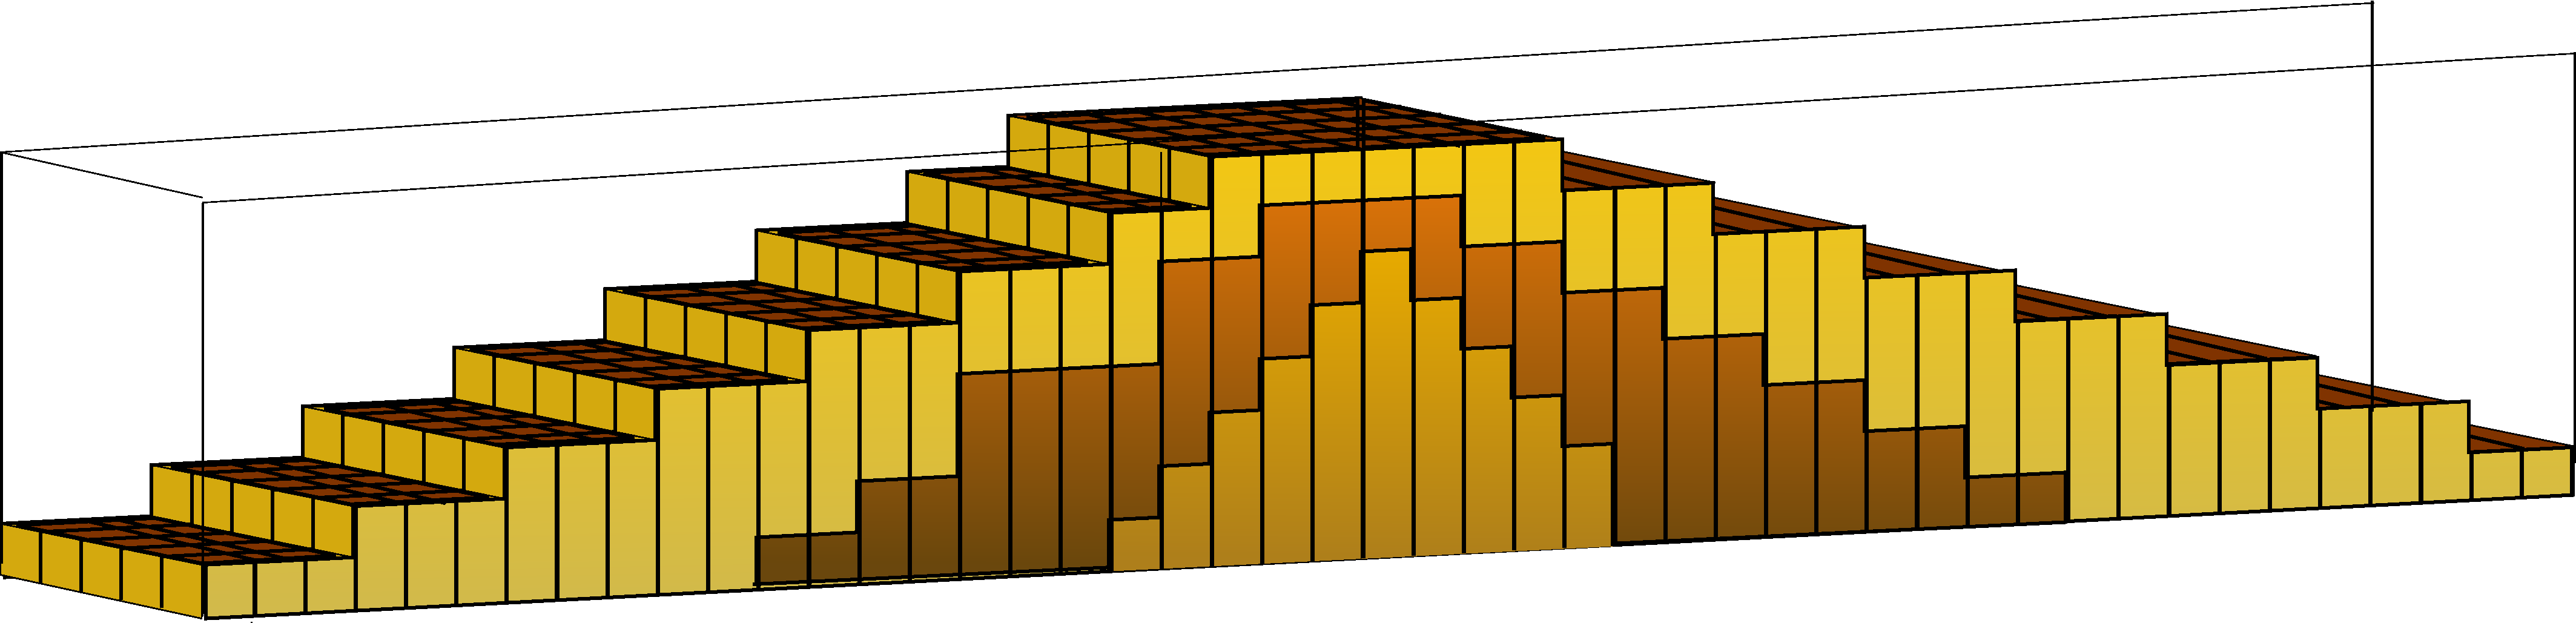
\includegraphics[width=1.0\textwidth, height=0.15\textheight]{images/SHF.pdf} 	 
    \end{minipage}
% 
   \begin{minipage}{0.49\textwidth}
    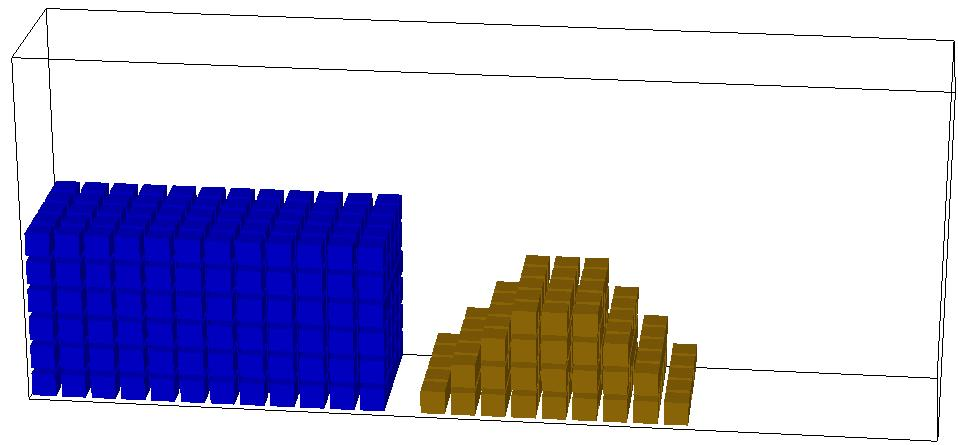
\includegraphics[width=1.0\textwidth]{images/VoxelGrid.jpg}
   \end{minipage}
% 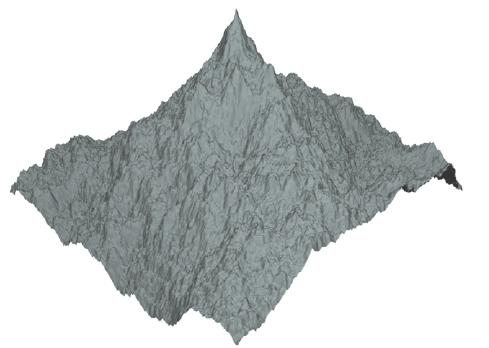
\includegraphics{images/HeightField.jpg} 
% 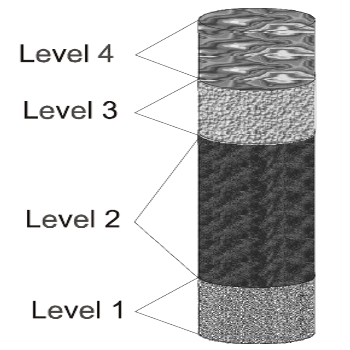
\includegraphics{images/LayeredDataRepresentation.png} 
	\caption[A rendering of volumetric terrain data structures]{(Left) 
% A rendered height field, in which the terrain is discretized into cells, each of which stores a single height. (Center) 
A layered height field, in which every grid space of the height field contains an array of arranged layers.
% similar to a height field except each cell contains an array of layers. 
(Right) A voxel grid, in which the terrain is constructed of cubes of materials, discretized in three dimensions.}
	\label{figure:data_structures}
\end{figure}

Many applications in computer graphics, such as erosion or weathering simulations, can be made more accurate and precise when terrain data is represented volumetrically. 

A voxel based terrain representation allows for immediate coupling with many fluid simulation techniques, as these are often based on a voxel grid (Figure \ref{figure:data_structures}). Fluid simulation (with terrain boundaries) using the Navier-Stokes equations is a straightforward application for a voxel grid, for instance. Voxel-based terrain representations allow for multiple materials, each with its own set of soil parameters, allowing for a more accurate simulation. Voxel grids allow for caves and undercuts as well because it is possible to model air as well as soil and fluid. Because of this, there is no limit to the fluid-soil boundary. Surface data is straightforward to draw from a voxel grid, but more importantly volume information is also inherent in the representation. Voxels also make complex renderings possible. However, voxel grids limit the precision of the terrain model, and the accuracy of the simulation is dependent upon the resolution of the grid in all three dimensions, as opposed to only two dimensions as for a height field. Voxel grids also require a lot of space to store, as well as connectivity information when dealing with soil layers.

Benes et al. \cite{Benes-LayeredDataRep} present a layered height field that combines several advantages of each of height fields and voxel grids. In their structure, the terrain is divided into a two dimensional grid, like a height field, but each grid space contains an array of heights (Figure \ref{figure:data_structures}). This representation allows for several different soil types, and a surface can be easily extracted for visualization and simulation purposes. The precision is arbitrary (to the degree of the computer's limit) because heights are stored as floating point values, which also significantly reduces storage. Most importantly, the layered representation allows for caves and undercuts by representing open air as one of the layers. The layered height field, however, does not allow for dynamic ordering of the layers, so new layers cannot be formed and if a particular soil type does not appear in a grid column then its value has zero depth, wasting space. If a dynamic implementation is used, new layers are added, then the newly added layer must be applied across the entire grid. Because sediment deposition may cause hundreds of layers to be added during a complex erosion simulation, this representation requires significant tuning before it is useful to us.

Some other representations have been used for terrain or similar models. Agarwala et al. \cite{argwala-Volume} present the ``slab'' data structure and use it for surface sculpting of volumetric models. Along the surface of the volume are assigned slabs, or small volumetric grids, that make local changes easier while not affecting the entire volume, thereby not requiring a global update. The slabs allow for updates to be made on a discrete grid structure while maintaining the underlying volumetric information of the rest of the model untouched by changes to the surface. The slabs are stored in quad-trees, allowing for local resolution adjustments as necessary by the level of detail required by a simulation. The authors use the slab data structure in the implementation of a surface sculpting simulation that requires only local updates when the surface is cut away. The authors also present a method for updating the rendering of the slabs by manipulating the display buffers to only update along the line of a stroke by a tool in the simulation. 
% This structure is too detailed for our purposes, but 
The idea of combining the benefits of many representations is an important one.

\section{Hydrography Network}
\label{section:PriorLiteratureChannelNetworkExtraction}

% \fbox{REWORD THESE, AND FIX THE CITATIONS}

An essential characteristic of terrain is its hydrography, consisting of the channel network (also known as its drainage or river network),
because hydraulic erosion is a prime factor in the
formation of terrain geometry.
% , particularly for levee breach events that motivate my work.
Accurate and efficient extraction of these networks
from DEM data has been an area of study for several
decades. It is essential for the analysis and comparison of terrains
as it allows for identification of channels, watersheds, valleys, and
drainage basins, but its challenges stem from the fact that the data
contains no information regarding the behavior of basins.
% 
Because of its importance, the pixels that make up the channels of the terrain's channel network 
are the focus of the placement of the drill operator. A great deal of attention in this 
work is paid to accurately extracting the channels.

%In 1984 
O'Callaghan and Mark \cite{OCALLAGHAN-Extraction} were among the first
to extract a channel network from a DEM, and their method is widely used in practice. 
% For each pixel of the terrain, the direction of the lowest of its eight neighbors is set as the flow direction. The pixels are sorted by elevation, and flow accumulation is calculated. 
Each pixel has its direction of flow calculated by determining the direction of steepest descent among its neighbors, and flow accumulation is calculated.
A threshold is applied to the accumulated flow values, and those pixels that surpass the threshold are considered part of the corresponding channel network.
% 
% This practice is widely
% used in channel network extraction, and finding the best
%ideal 
% threshold for a particular terrain
%to use on a channel network is the basis of our work.
% is one of the specific objectives discussed in this thesis. 
In this method, slight variations in geometry could render a threshold significantly less useful.
% , and so when dealing with sequential data an adaptive threshold is vital. 
Comparing two terrains only makes sense if they have similar channel networks, 
and so identifying optimal thresholds 
% that minimize the difference between the extracted networks 
is an important research question.

In addition, elevation tie-breaking (in the case of an elevation tie between neighboring pixels, such as in basins, determining which pixel is ``lower'' for the purposes of the flow algorithm) and how pits are dealt with continue to be challenging research questions, as the methods used have a surprisingly strong effects on the extracted channel network.

%In 1986, 
L. Band \cite{band86} describes a method for extending O'Callaghan and
Mark's work to identify channel watersheds by grouping pixels that
flow into the same channel. To minimize the need for tie-breaking procedures, grouped pixels are treated as a single pixel.
% Once grouped, they can act as a single pixel and can accumulate flow as one, thus minimizing the need for tie breaking. 
However, this does not solve the problem of flat basins completely.
%In 1997, 
Yang et al. \cite{YANG-geomorphic} describe the effect various
thresholds have on two widely used watershed analysis tools, the {\em
  width function} and the {\em area function}, finding that at low
thresholds the two measures are similar but vary greatly as thresholds
increase and channel networks shrink. 
%In 1993, 
Montgomery and Foufoula \cite{MONTGOMERY-1993} present a
comparison between 
two channel network calculation models, the constant threshold and the slope-dependent models.
% the constant threshold and slope-dependent models
% for calculating channel networks, presenting 
They find that each
method appears valid in certain instances. They also describe a method
for identifying channel heads as a means for extracting channels.

Other methods for channel network extraction have required additional
input. Turcotte et
al. \cite{Turcotte_Fortin_Rousseau_Massicotte_Villeneuve_2001}
introduce the {\em Digital River and Lake Network}, which is required
as input in addition to a DEM. This allows for the handling of lakes
in the terrain, a source of frustration for previous methods because
of the difficulty of tie-breaking procedures.

%  and the lake of flow volume. 
Some methods have foregone flow calculation entirely and
depended upon the geometry of the terrain surface exclusively, such as
Lashermes et al. \cite{Bruno2007}, who present a method for
extracting valleys and hills from a terrain using wavelet filtering on
high resolution DEMs.  Still other methods have attempted to define
characteristics on the terrain. Kramer and
Marder~\cite{PhysRevLett.68.205} use a shallow water simulation to
model the flow of water over the terrain, measuring the formation of
channels with the area and width functions. Similarly, Soille et
al.~\cite{Soille_carvingand} overcome the tie-breaking dilemma in
network extraction by running a flooding simulation to create a path
through pits in the terrain. However, in both of these methods computation
costs make analysis of large terrains difficult.


\section{Terrain Data Compression}
\label{section:TerrainDataCompression}

Terrain data compression is an obvious yet vital application of novel terrain representations. Many representations are specifically designed to be easily compressed, while other schemes take advantage of the characteristics of the more popular representations. The characteristics of terrain that compression schemes should work to retain go beyond simple height values. While it is hard to be absolutely sure of the accurate hydrography data given a terrain dataset (which contains errors due to data collection itself), schemes that ignore this property can easily compound error in what is a critical characteristic of the terrain surface. For this reason, research into compression schemes is varied and extensive.

There are two types of compression: \textit{lossy} and \textit{lossless}. Lossy compression sacrifices some data for a higher compression ratio, whereas no data is lost due to lossless compression. \textit{Near-lossless} compression refers to a scheme that allows the user to bound the error of the regenerated data, meaning that it can be lossless if the user elects to have the bound on the error be 0\%.

\subsection{Compressing Terrain Features}

One of the primary methods for compression is to select the most ``important'' elements of the data and store only them. Pedrini \cite{conf/wscg/Pedrini01} presents a method for building a terrain surface from a set of data points. It alternates between refinement and decimation steps, meaning that a set of points is selected to represent the surface, and then a set of less useful ones are removed from the chosen set, and the process is repeated until a global error threshold is met. Dyn et al. \cite{Dyn02adaptivethinning} present a method for thinning a dataset based on the error present in the triangulation of the points, which entails removing points one-by-one and recalculating the error until a global threshold is met. The algorithm presented works with several triangulation and error calculation techniques. Kolar \cite{1e218e70004511dab4d5000ea68e967b} presents a method for building a level-of-detail hierarchy of triangle vertices using the idea of ``mass points'', or vertices that are assigned to levels in the hierarchy based on the frequency of the terrain around them. 

Similarly, Xie et al. \cite{Xie_approximatingterrain} present the ODETLAP algorithm, which treats a matrix of elevation values (with holes) as an overdetermined Laplacian system with equations for each known elevation value. This allows for a selective compression scheme since an incomplete surface can be rebuilt using ODETLAP, and so only the most ``important'' points are stored. 
This method is also presented by Inanc \cite{inanc-phd}. In his work, Inanc presents the ODETCOM system, which obtains near-lossless 
% (lossy compression whose error is user-bounded) 
compression with good results. Like ODETLAP, ODETCOM creates and overdetermined system of equations using a predictor model. The predictor is based on a template whose size is variable depending upon a desired accuracy threshold, creating a near-lossless scheme.

Pradhan et al. \cite{Pradhan_gisterrain} present a method of compression terrain data that uses a Delaunay triangulation, and a "lifting technique" to compress. During the lifting, each triangle is divided into smaller triangles, allowing each level of the compression to be written as its own wavelet equation, which is then encoded. Along those lines, Kim et al. \cite{Kim_ageometric} present an algorithm for compressing Delaunay triangulations of a series of 2.5D points (that describe a surface). The algorithm revolves around finding both the Delaunay triangulation and any other single triangulation, and defining the ex-or function that finds the set of vertices and edges not in the intersection of both triangulations.
% , achieving good results.
%  The paper introduces a series of theorems about the comparison of triangulations and subgraphs of said triangulations.

\subsection{Image Compression}
\label{subsection:ImageCompression}

Because height field 
% and TIN 
representations of terrain are isometric to greyscale image data, image compression techniques are often used to compress terrains. Grazzini and Chrysoulakis \cite{Grazzini05n.:extraction} take advantage of this characteristic by noting that traditional features of terrain, such as slope, aspect, and curvature, are not scale invariant, and thus do not fit the needs of all representations. And so they present a terrain feature extraction method for greyscale images using a multifractal representation of image data. 

Image compression techniques ignore many of the features found on terrain, and do not take advantage of the characteristics of terrain that many terrain-specific compression schemes do. However, from a purely statistical standpoint,  they are more successful in general with regard to compression ratios. There are many families of image compression schemes, the most widely used being JPEG and PNG.
% , and medical image compressions.

JPEG (named after the group that created it: Joint Photographic Experts Group) \cite{Penn92}
is the industry standard for lossy image compression, and consists of a series of steps to transform, downsample, and quantize image information before encoding. 
The algorithm divides the image into a series of smaller blocks (8 x 8 groups of pixels) that it treats as matrices that are transformed to the frequency domain via the Discrete Cosine Transform. The result of this transform can be truncated and encoded, which provides for the compression.
% The process works by identifying blocks of pixels with similar chrominance and downsampling to reduce redundancy. The scheme works well in a terrain domain because neighboring pixels often share similar elevations, or intensity values in image space, which allows for large blocks to be identified and encoded.
JPEG compression often obtains 20:1 compression ratios with no noticeable degradation to quality. This serves as a good baseline comparison for terrain compression schemes.
% 
A variation on JPEG, called JPEG-2000 \cite{Taubman:2001:JIC:559856}, is a lossless scheme that takes advantage of wavelets to compress image data.

PNG (Portable Network Graphics) image compression \cite{316738} creates a string of sequential differences between color values of the pixels of the image. Storing the first pixel value and then a series of distances creates a situation in which homogeneous sections (with several 0s in a row) can be compressed effectively with run length encoding, or other similar schemes. PNG compression is lossless, but like many lossless schemes can be converted to a lossy scheme by sacrificing some accuracy by sampling, obtaining a better compression ratio.

The JBIG compression scheme \cite{Kyrki99jbigimage} was designed for binary images and uses IBM's Q-Coder arithmetic coder to encode each pixel, a function of its immediate neighborhood. A greyscale (or even color) image can be compressed by acting on a single bit plane at a time (i.e., treat an 8-bit-per-pixel greyscale image as 8 separate binary images). 

Dozens of other compression schemes exist for images. Some are optimized for greyscale images, some for color, and some specialize in specific kind of images, such as medical images (Zukoski et al.\cite{Zukoski:2006:NAM:1356588.1356594}, Raj and Venkateswarlu \cite{Raj:2007:NAM:1335117.1335447}, for example).
% 
It is difficult to best standard image compression schemes with regard to compression ratio. The primary goal of terrain data compression is meeting an accuracy threshold with as high a compression ratio as possible. A lossy image compression scheme may result in small elevation errors that exacerbate the error in the hydrography of the regenerated terrain surface. As such, they are not necessarily ideal, despite their superior compression ratios. 

% \fbox{FINISH THIS SECTION WITH A MORE EXAMPLES}


% \section{Shape Analysis Techniques}
% \label{section:ShapeAnalysisTechniques}
% 
% In order to judge the accuracy of terrain representations and compression schemes (or any application in which there is an attempt to match spatial data),
% % such as a height field), 
% a method for determining a ``distance'', or measure of dissimilarity, between two 
% % terrain
% datasets is used. One way in which this is accomplished is through shape analysis.
% % \subsubsection{Using Shape Analysis}
% 
% Shape analysis has been studied in computer graphics and computer vision
% for decades, most often used in shape
% matching and pattern recognition. Shape matching is the process of choosing,
%  from a set of possible partners,
%  the closest to a given shape, while pattern recognition is a computer vision
% problem involving picking out examples of a given shape in an image or scene. 
% Shape matching relies on difference metrics, measures of the dissimilarity
% between two shapes. The smaller the dissimilarity, the closer the two
% shapes are to one another.
% 
% Treating terrains and their associated channel networks as shapes is a
% method for comparison from which distance metrics arise naturally. Fundamentally
% the goal is to be able to compare the shapes of the extracted channel networks.
% % that are extracted from terrain data. 
% 
% Often, shape dissimilarity metrics
% are used as bases for finding the correlation between shapes, if one
% exists.  Belongie et al.~\cite{belongie-ShapeContexts} present the
% idea of ``Shape Contexts'', in which a two dimensional shape is
% described by the angle to the X-axis of the tangent of every point along the border of the shape. In this instance, the X$_{2}$ metric can be used as the
% dissimilarity measure between the shapes. An
% extension~\cite{Belongie:2002:SMO:628328.628792}
% to this idea broadens
% the criteria for the shape context by basing its measure on the shape's angle relative to the
% tangent along the shape border instead of the X-axis,
%  making the shape
% context operation invariant under rotation.
% 
% Shape comparison was later applied to three dimensions 
% by Osada~\cite{Osada-ShapeDistributions}, who presents the idea of
% representing three dimensional shapes as a probability
% distribution. Given any shape distribution function (such as the
% \emph{D2} function, a measure of Euclidean distance between two random
% points on the shape surface), the authors build a probability distribution
% function of the shape by selecting random points along the
% surface. These probability distributions can then be compared and
% analyzed by any known means.
% 
% Roy et al.~\cite{Roy04meshcomparison} provide a metric for comparing
% triangle meshes. For each sampled point on the first mesh and a given
% shape attribute, the method finds the closest point of the same
% attribute in the comparison mesh. Geiger et
% al.~\cite{Geiger:2003:RSS:628334.628872} find the Shape Axis tree
% (first presented in Luh and Geifer~\cite{Luh-791256}) and use an
% optimization function to find self-similarity in shapes. They identify
% the best match between two spline curves, one representing the
% parameterized shape and the other representing the shape parameterized
% in reverse. 
% Gal et al.~\cite{10.1109/TVCG.2007.45} present a new
% pose-oblivious shape signature function that defines the overall
% topography of a shape. This is achieved through use of the local
% diameter function and the centricity function, in which the distance between the mesh and a ray
% shot perpendicular to the normal at a point along the mesh is
% measured.  The second function is a measure
% of the average geodesic distance from a point on the mesh to every
% other point on the mesh.  
% Mademlis et
% al.~\cite{Mademlis-ShapeRetrieval} describe a method for shape
% retrieval by matching shapes with those in a database. The algorithm
% segments the shapes, and builds a probability matrix for each segment
% of each shaping, defining the probability that segment $i$ in one shape
% matches segment $j$ in the other. 
% By applying a metric to this
% probability matrix, they determine the likelihood that the two shapes
% match.
% 
% Shape analysis has also been used for animation and deformations.
% M\"ueller et al.~\cite{Muller:2005:MDB:1186822.1073216} present a
% simulation of deformable objects by creating a \emph{goal state} for
% the mesh and minimizing the total energy required to deform the mesh
% to the goal state. Correspondences between points on the current and
% goal states are found through shape matching algorithms. Huang et
% al.~\cite{10.1109/3DIM.2007.8} compare the performance of four
% well-known shape dissimilarity metrics, testing frames in three
% different human animations.
% 
% 
% 
% % These methods provide a useful basis for comparing two meshes,
% % including height fields. However, my needs revolve around specific
% % aspects of the terrains, namely the channel network. To the best of
% % my knowledge, no shape analysis tools have been specifically applied
% % to height field data in computer science literature. In my work, we
% % use variations on the Hausdorff distance, as well as direct pixel to
% % pixel comparisons, to determine the distance between two channel
% % networks, a vital process for terrain comparison and failure
% % diagnosis.



\section{Summary of Prior Art in Terrain Modeling}

Existing spatial representations of terrain data include height fields, TINs, 
and splines. These spatial models fail to accurately represent complex surface features, such as 
caves and cliff faces, which introduce surface discontinuities. 
% 
Volumetric representations, such as voxel grids, are capable of representing
these features, but with too large of a memory footprint to be practically
useful in many GIS applications. 
% 
In addition, none of these representations maintain ties to the hydraulic
erosion responsible for the formation of the terrain, ignoring the hydrography
of the surface.
% 

Hydrographically valid terrains are important for a variety of GIS applications, including many that require the extraction of an accurate and suitable channel network. These include path planning, dam siting, and observer siting algorithms, among others. GIS lacks a procedural representation of terrain whose formation guarantees hydrographic validity by removing local minima and allowing the encoding of complex terrain features.
Until such a representation exists, there is little need to work toward more accurate and robust data collection procedures.

Many data compression techniques, such as feature or image compression, ignore the need to maintain hydrographically valid terrain data, as well. These schemes, while accomplishing substantial compression ratios, fail to maintain important features, and are not tied to any specific representation or formation procedure.

% The surface's hydrography network, or channel network, can be extracted from the surface
% using a variety of methods. Some require pre-processing the terrain, such as filling in 
% pits. Others find the least-cost path from a pixel to the edge of the terrain. 

Moving toward more accurate terrain data collection and storage requires
a representation of the terrain surface that is capable of overcoming these
shortcomings. 
% 
The drill operator, presented in Chapter \ref{chapter:DrillOperator},
has been designed with this goal in mind.









